\chapter{Analisi dei requisiti}
\label{analisi}

\section{Modello di Dominio}
\begin{figure}[H]
	\centering
	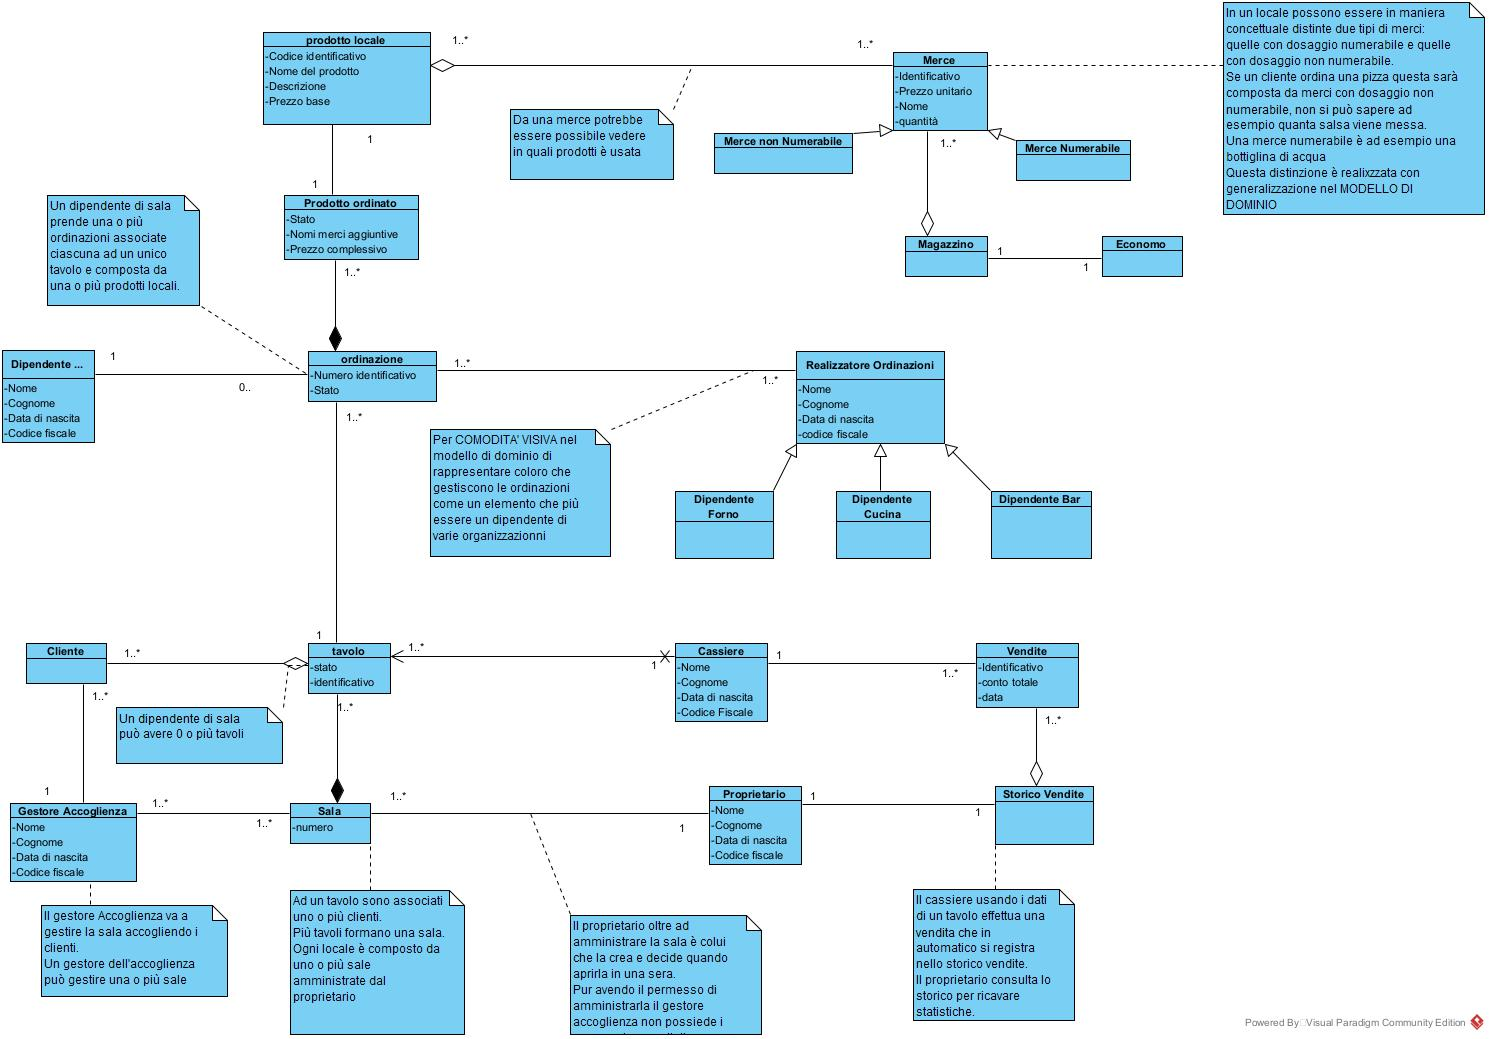
\includegraphics[width=1\textwidth]{Immagini/modello_dominio.jpg}
\end{figure}
Con questo primo diagramma di analisi si sono fatte le prime ipotesi di funzionamento (descritte dai commenti), mettendo in evidenza le relazioni tra le varie entità del sistema.

\begin{enumerate}
	\item In un locale con più camerieri si può verificare la situazione in cui diversi camerieri possono prendere le ordinazioni ad uno stesso tavolo. Con questa ipotesi quindi il cameriere non viene associato direttamente al tavolo, ma all'ordinazione che ha creato per esso.
	\item Il sistema gestisce le merci in modo automatizzato. Esse sono divise in \textit{numerabili} e \textit{non numerabili}. A tal proposito, quando il cameriere crea un'ordinazione che contiene delle merci numerabili, esse vengono immediatamente scalate dal magazzino.
	\item Tutte le vendite completate vengono memorizzate in uno storico.
	\item Il prodotto che viene aggiunto all'ordinazione non equivale al prodotto presente nel menu. Esso infatti può subire delle modifiche come aggiunta o rimozioni di merce dalla sua versione di base. Viene indicato quindi come l'entità \textit{Prodotto Ordinato}.
\end{enumerate}

\section{State Chart Diagram}
Alcune entità del sistema hanno delle funzionalità diverse in relazione allo stato in cui si trovano.

\subsection{Tavolo}
\begin{figure}[H]
	\centering
	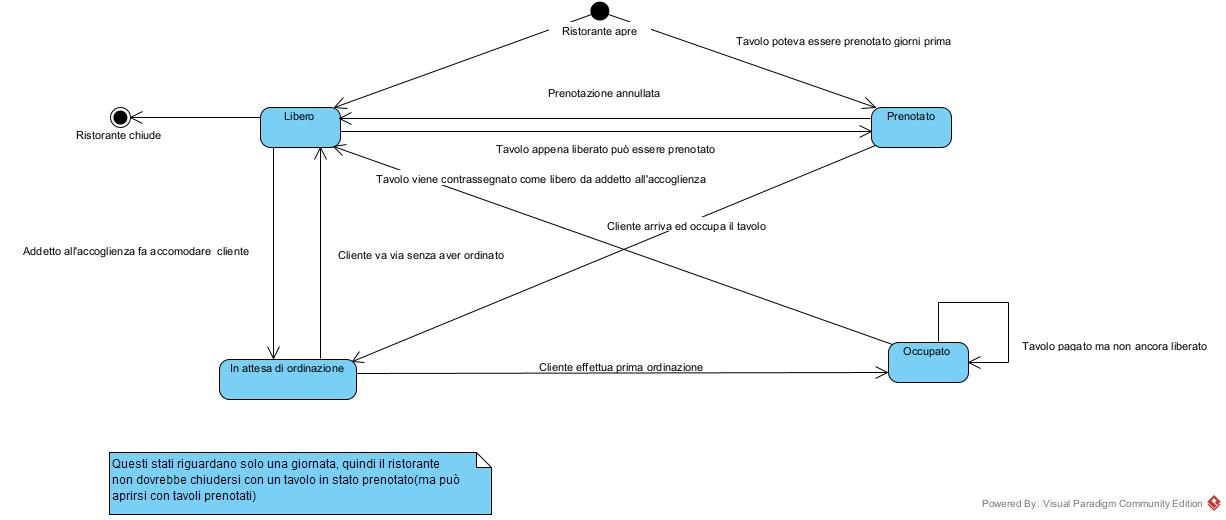
\includegraphics[width=1\textwidth]{Immagini/stati_tavolo.jpg}
\end{figure}
Questi stati valgono solo durante l'esecuzione del sistema. In teoria il locale non può chiudere con tavoli occupati o in attesa di ordinazione. Attraverso questi stati esiste anche più controllo per evitare errori umani. Ad esempio un cameriere non può prendere le ordinazioni di un tavolo libero, ovvero non occupato da nessun cliente.

\subsection{Prodotto Ordinato}
\begin{figure}[H]
	\centering
	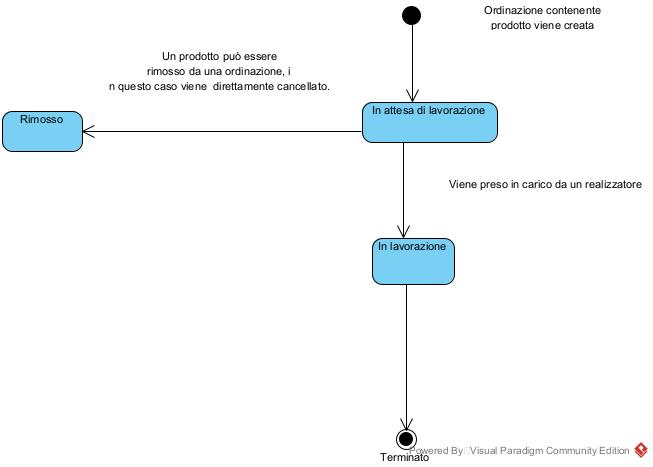
\includegraphics[width=0.8\textwidth]{Immagini/stati_prodotti_ordinati.jpg}
\end{figure}
Gli stati vengono aggiornati tramite dei feedback di chi realizza i relativi prodotti.

\subsection{Ordine}
\begin{figure}[H]
	\centering
	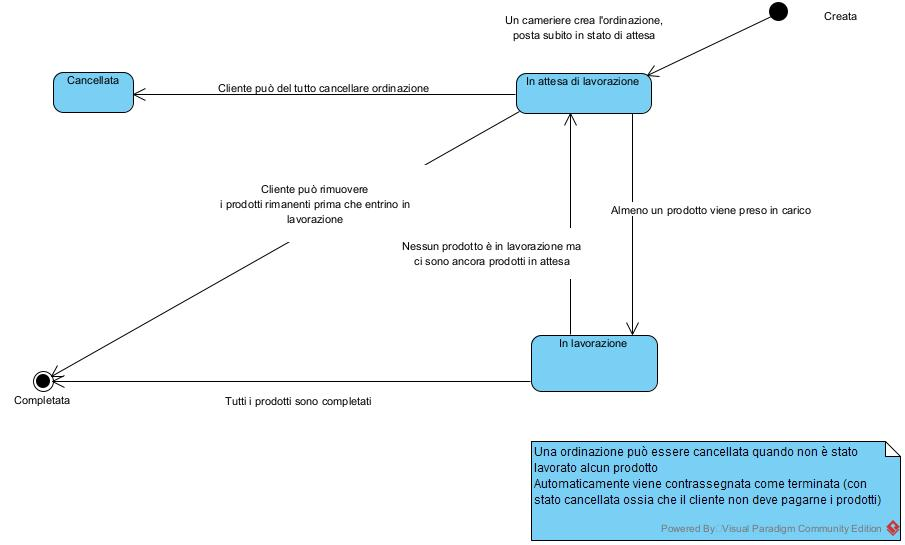
\includegraphics[width=1\textwidth]{Immagini/stati_ordinazione.jpg}
\end{figure}
Gli stati dell'ordine dipendono molto dagli stati dei prodotti ordinati che lo compongono, essendo infatti un'aggregazione di prodotti.

\section{Sequence Diagram di Dominio}
I seguenti sequence diagram sono realizzati solo per indicare le interazioni tra un utente e il sistema.

\subsection{Gestisci Ordinazioni}
\subsubsection{Estensione A}
\begin{figure}[H]
	\centering
	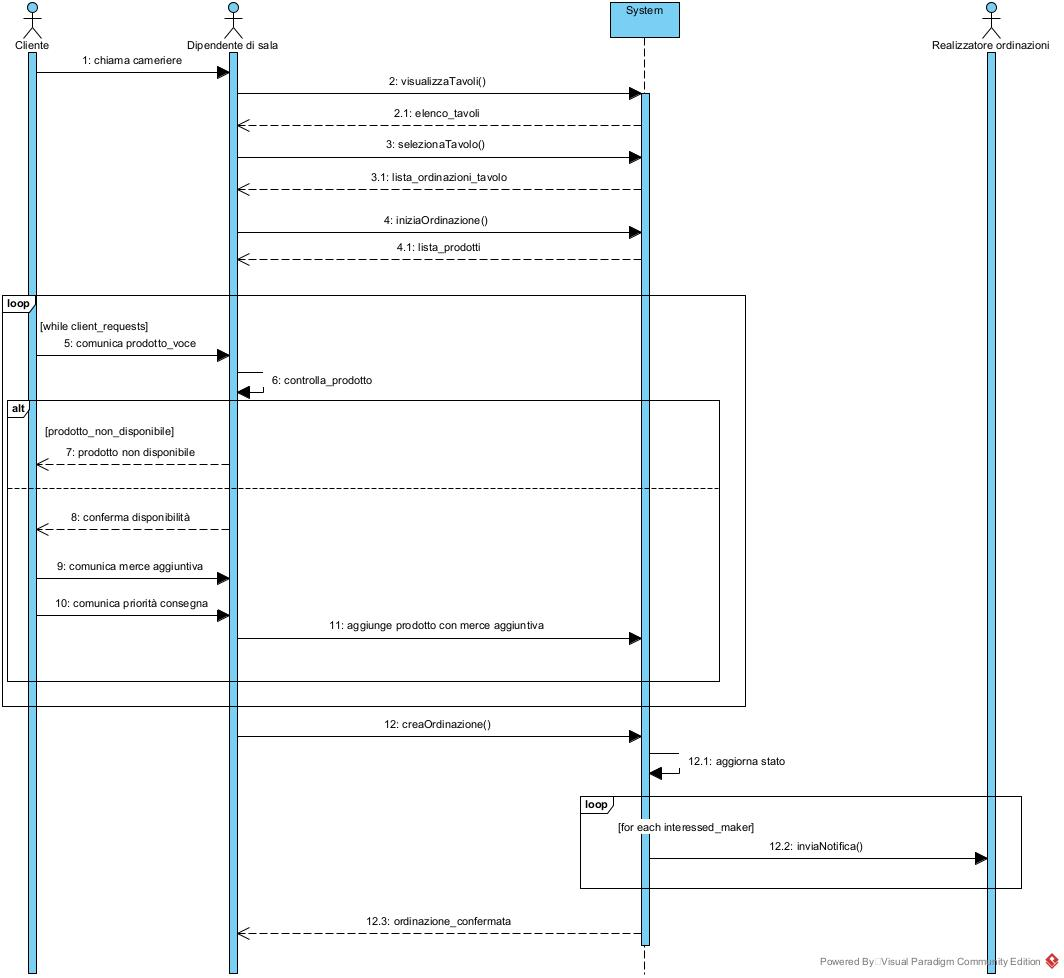
\includegraphics[width=1\textwidth]{Immagini/SSD Gestisci Ordinazioni (Successo).jpg}
\end{figure}

\subsubsection{Estensione B}
\begin{figure}[H]
	\centering
	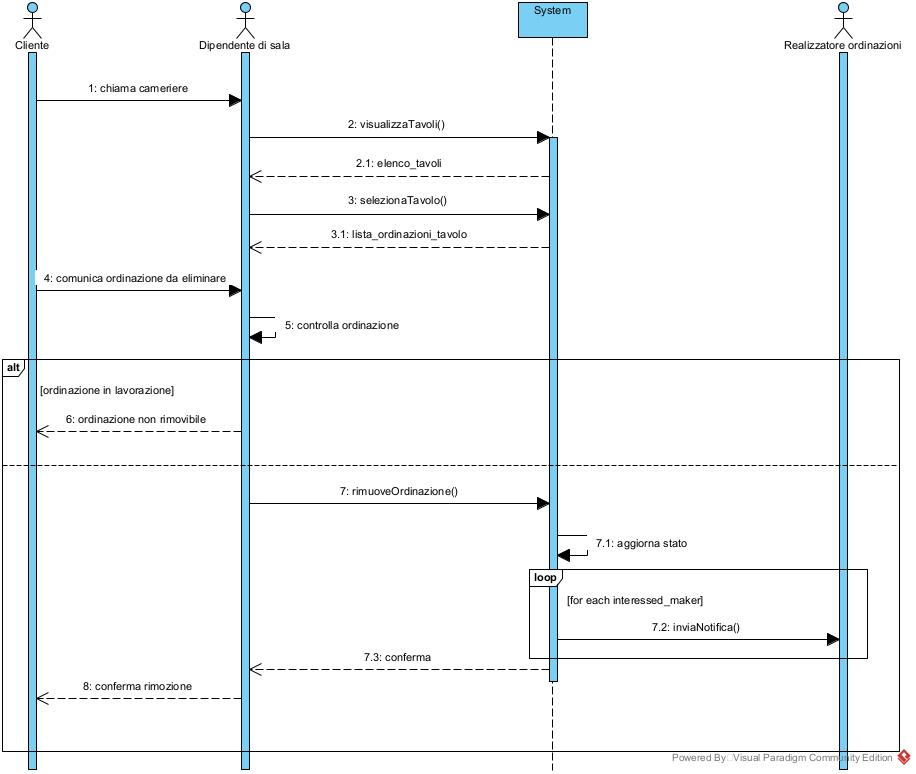
\includegraphics[width=1\textwidth]{Immagini/SSD Gestisci Ordinazione (EstensioneB - Elimina Ordinazione).jpg}
\end{figure}

\subsubsection{Estensione C}
\begin{figure}[H]
	\centering
	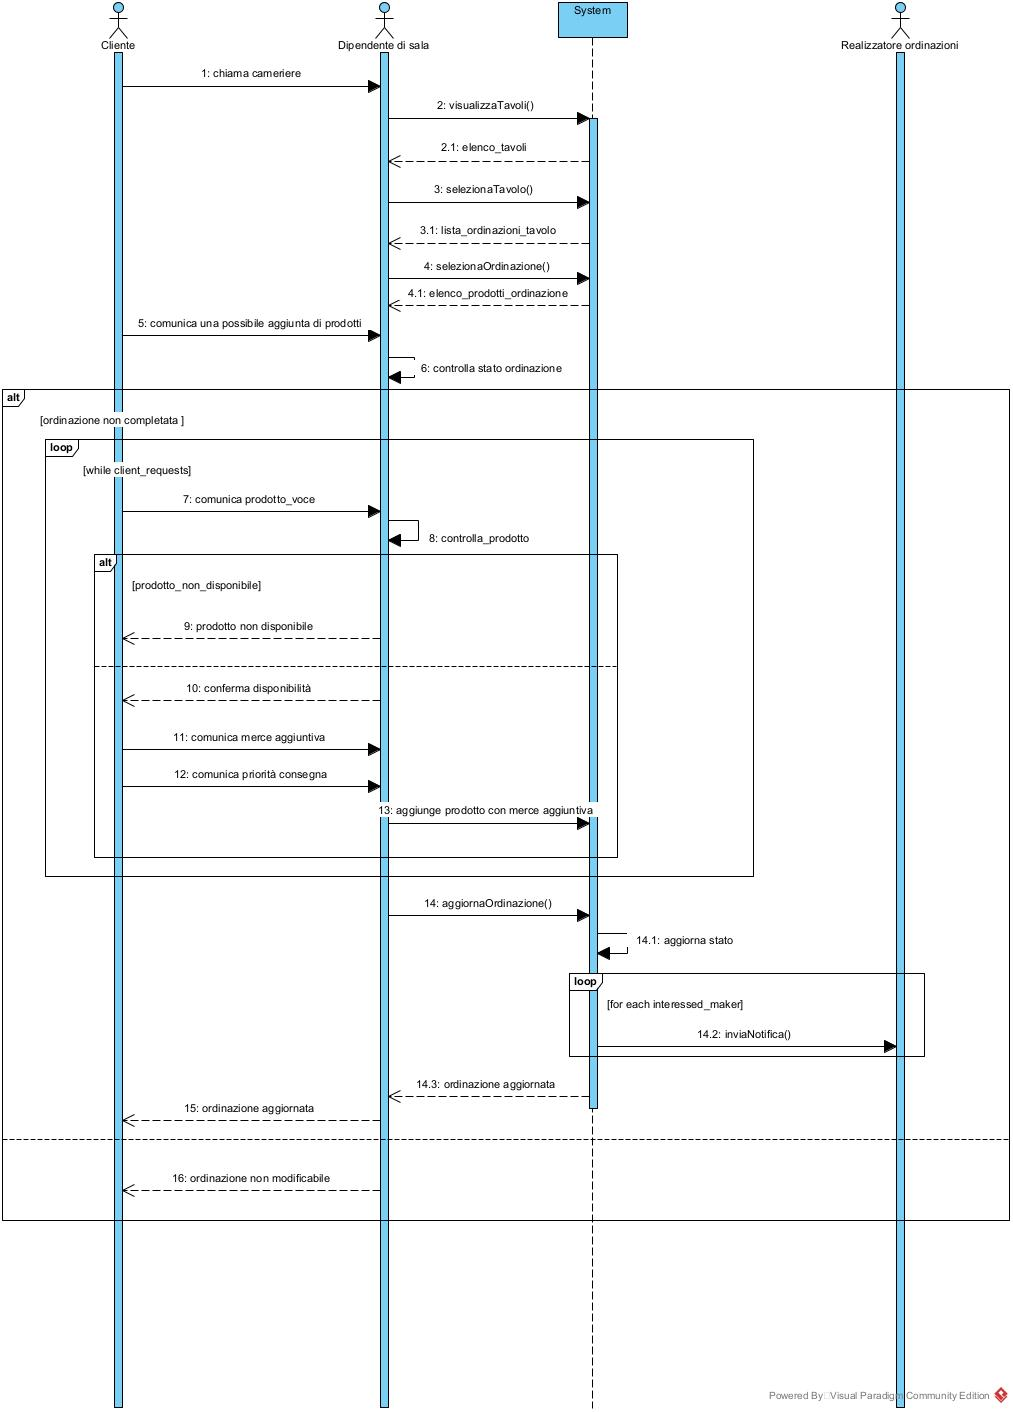
\includegraphics[width=1\textwidth]{Immagini/SSD Gestisci Ordinazione (EstensioneC - Aggiungi prodotto).jpg}
\end{figure}

\subsubsection{Estensione D}
\begin{figure}[H]
	\centering
	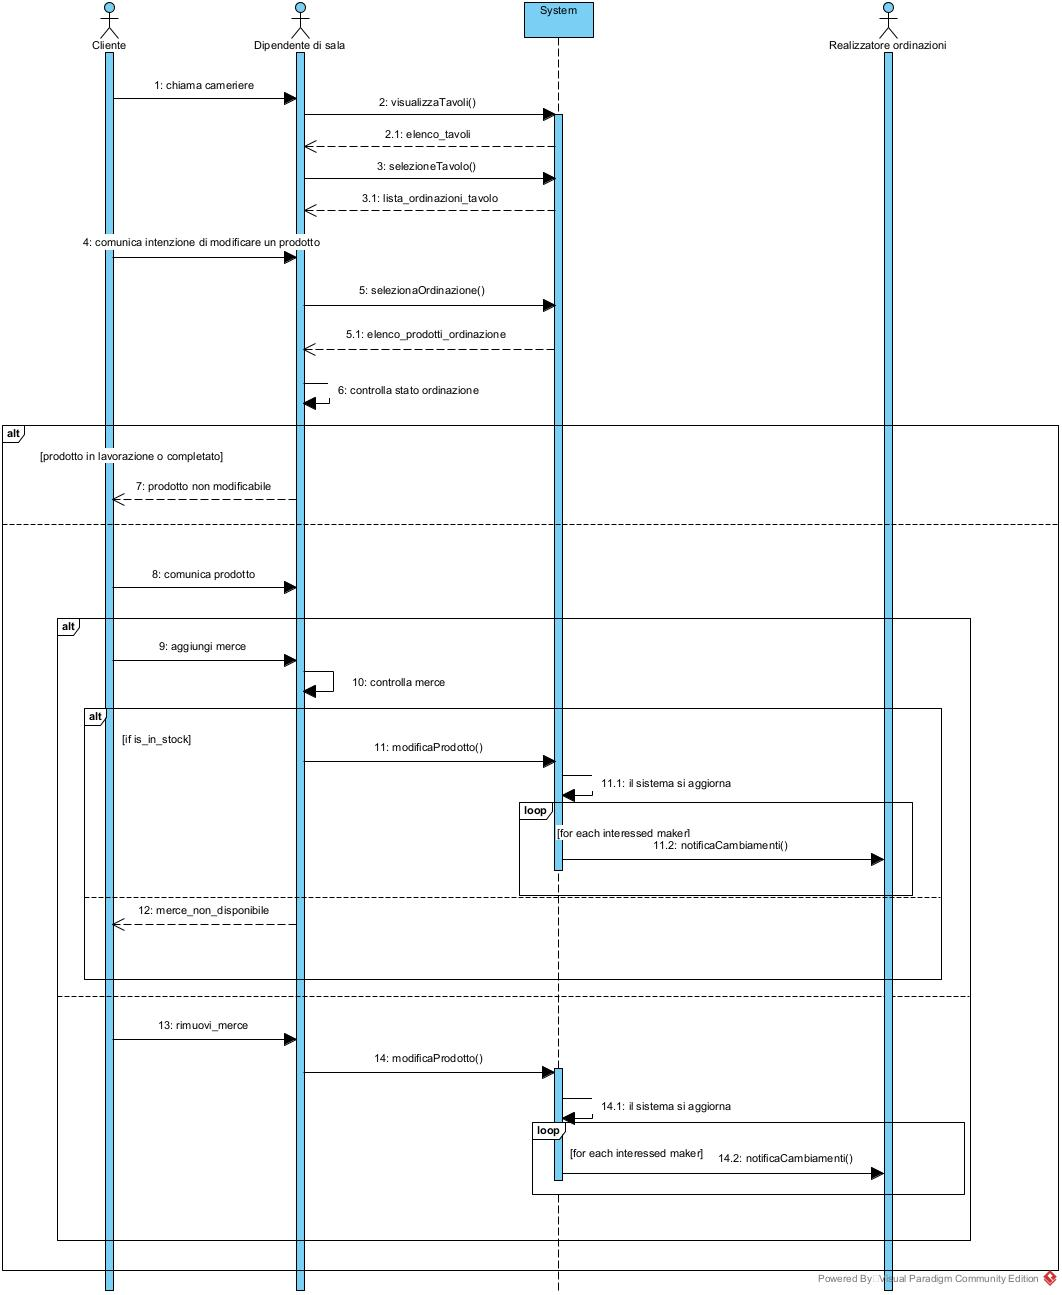
\includegraphics[width=1\textwidth]{Immagini/SSD Gestisci Ordinazione (EstensioneD - Modifica prodotto).jpg}
\end{figure}

\subsubsection{Estensione E}
\begin{figure}[H]
	\centering
	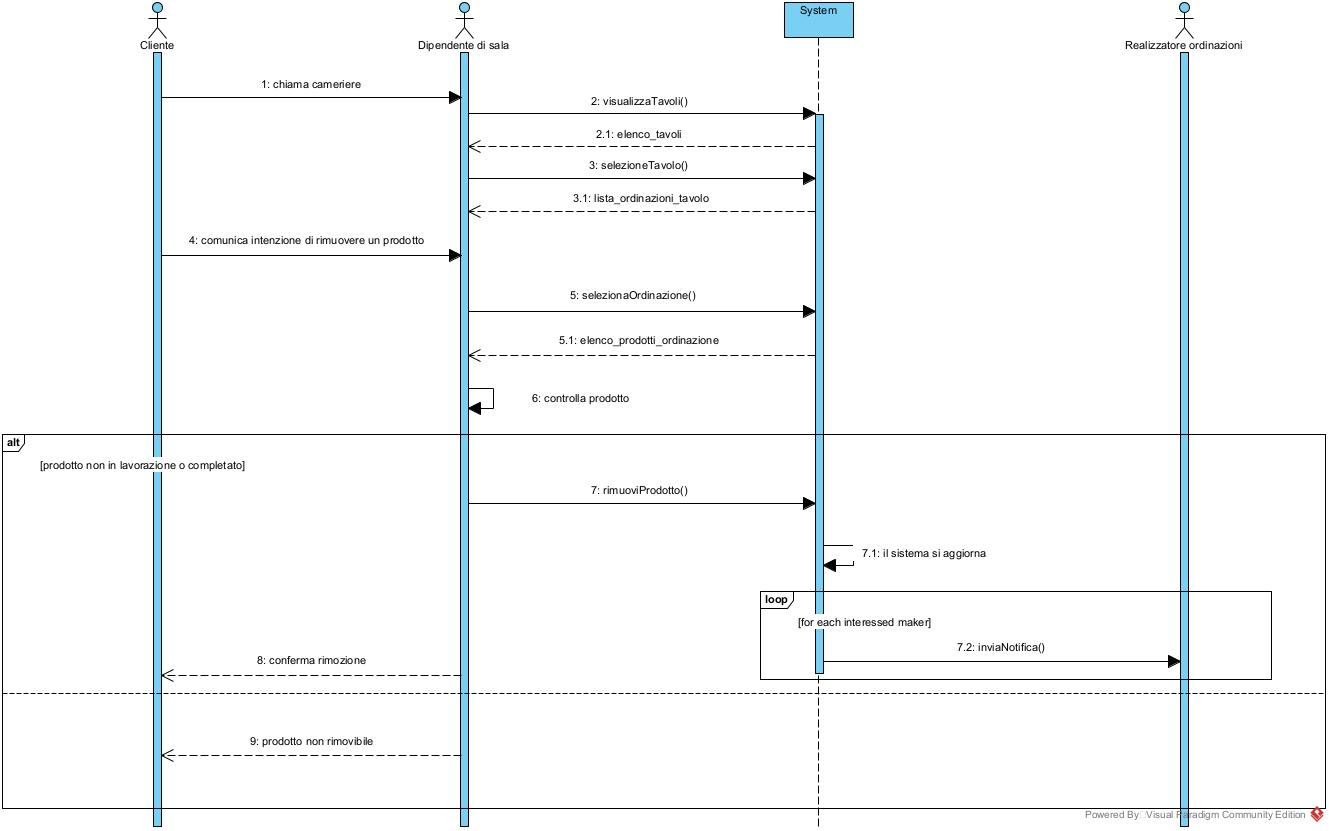
\includegraphics[width=1\textwidth]{Immagini/SSD Gestisci Ordinazioni (Estensione E - Rimuovi prodotto ordinazione).jpg}
\end{figure}

\subsection{Notifica Ordinazione}
\subsubsection{Estensione A}
\begin{figure}[H]
	\centering
	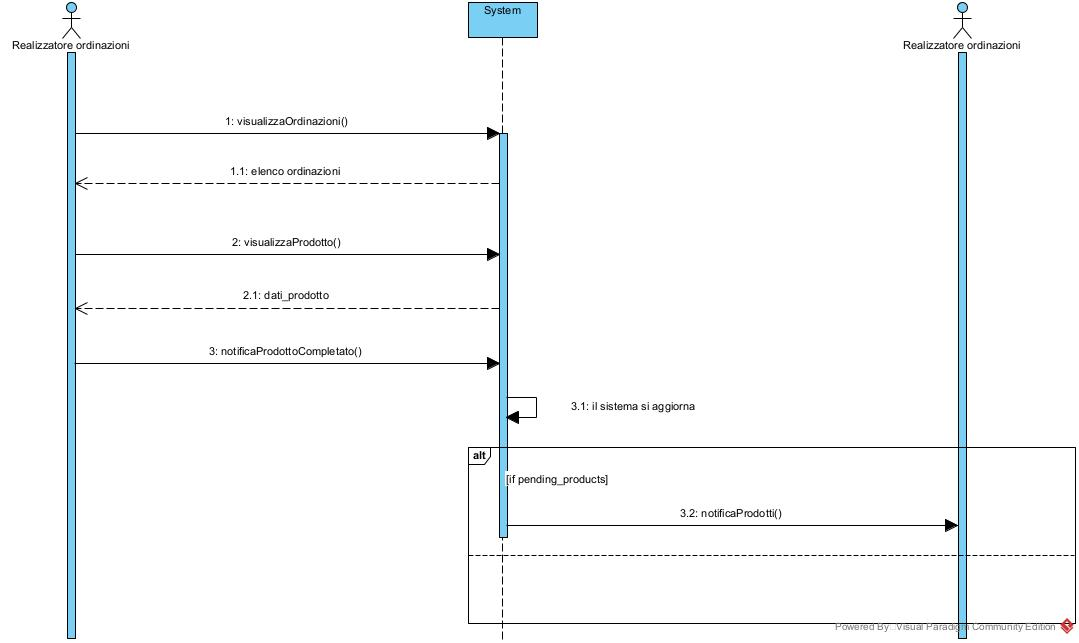
\includegraphics[width=1\textwidth]{Immagini/SSD Notifica Ordinazione.jpg}
\end{figure}
